\section{Kết quả và Thảo luận}

Phần này trình bày các kết quả thực nghiệm thu được, so sánh hiệu năng giữa mô hình cơ sở và mô hình sau khi tinh chỉnh, đồng thời thảo luận về các ưu điểm và hạn chế của phương pháp đề xuất.

\subsection{Phương pháp đánh giá}

Hiệu năng của mô hình được đánh giá dựa trên hai chỉ số tiêu chuẩn trong bài toán OCR:

\begin{itemize}
    \item \textbf{CER (Character Error Rate):} Tỷ lệ lỗi ký tự, được tính bằng khoảng cách Levenshtein giữa chuỗi ký tự dự đoán và chuỗi nhãn gốc, chia cho độ dài của chuỗi nhãn.
    \begin{equation}
        CER = \frac{S + D + I}{N}
    \end{equation}
    Trong đó: $S$ là số phép thay thế (substitutions), $D$ là số phép xóa (deletions), $I$ là số phép chèn (insertions), và $N$ là tổng số ký tự trong nhãn gốc. Chỉ số này đặc biệt quan trọng đối với tiếng Việt vì sự hiện diện dày đặc của các dấu phụ và dấu thanh.

    \item \textbf{WER (Word Error Rate):} Tỷ lệ lỗi từ, được tính toán tương tự như CER nhưng trên đơn vị từ. WER phản ánh khả năng nhận dạng đúng toàn bộ từ vựng, điều này rất quan trọng cho các tác vụ xử lý ngôn ngữ tự nhiên tiếp theo.
\end{itemize}

\subsection{Kết quả định lượng}

Chúng tôi tiến hành đánh giá và so sánh hiệu năng giữa mô hình cơ sở (Baseline - Zero-shot) và mô hình sau khi tinh chỉnh (Fine-tuned) trên tập kiểm tra độc lập (Test set).

\begin{table}[H]
\centering
\caption{So sánh kết quả giữa mô hình Baseline và Fine-tuned trên tập kiểm tra}
\begin{tabular}{|l|c|c|}
\hline
\textbf{Mô hình} & \textbf{CER (\%)} & \textbf{WER (\%)} \\
\hline
Baseline (Zero-shot) & 23.599466 & 2.816725 \\
\hline
Fine-tuned (Ours) & 0.475978 & 0.733551 \\
\hline
\textbf{Cải thiện} & \textbf{23.123488} & \textbf{2.083174} \\
\hline
\end{tabular}
\end{table}

\textit{(Lưu ý: Các con số cụ thể sẽ được cập nhật sau khi hoàn tất quá trình chạy thực nghiệm trên toàn bộ tập kiểm tra.)}

\subsection{Thảo luận và Phân tích lỗi}

\subsubsection{Cải thiện so với Baseline}
Kết quả thực nghiệm cho thấy mô hình sau khi tinh chỉnh (Fine-tuned) đạt được sự cải thiện vượt bậc so với mô hình Baseline.
\begin{itemize}
    \item \textbf{Nhận dạng dấu tiếng Việt:} Mô hình Baseline thường gặp khó khăn trong việc phân biệt các dấu thanh nhỏ (như dấu nặng, dấu huyền) hoặc bỏ qua hoàn toàn các dấu mũ (â, ê, ô). Mô hình Fine-tuned đã khắc phục được phần lớn các lỗi này, nhận dạng chính xác các ký tự có dấu phức tạp.
    \item \textbf{Xử lý nét viết tay:} Với dữ liệu chữ viết tay tự do (unconstrained handwriting), nét chữ thường biến dạng, nghiêng hoặc dính vào nhau. Mô hình Fine-tuned thể hiện khả năng thích nghi tốt, phân tách và nhận dạng đúng các ký tự viết tháu.
\end{itemize}

Các hình dưới đây minh họa một số trường hợp điển hình mà mô hình Fine-tuned đã cải thiện đáng kể so với mô hình Baseline:

\begin{figure}[H]
    \centering
    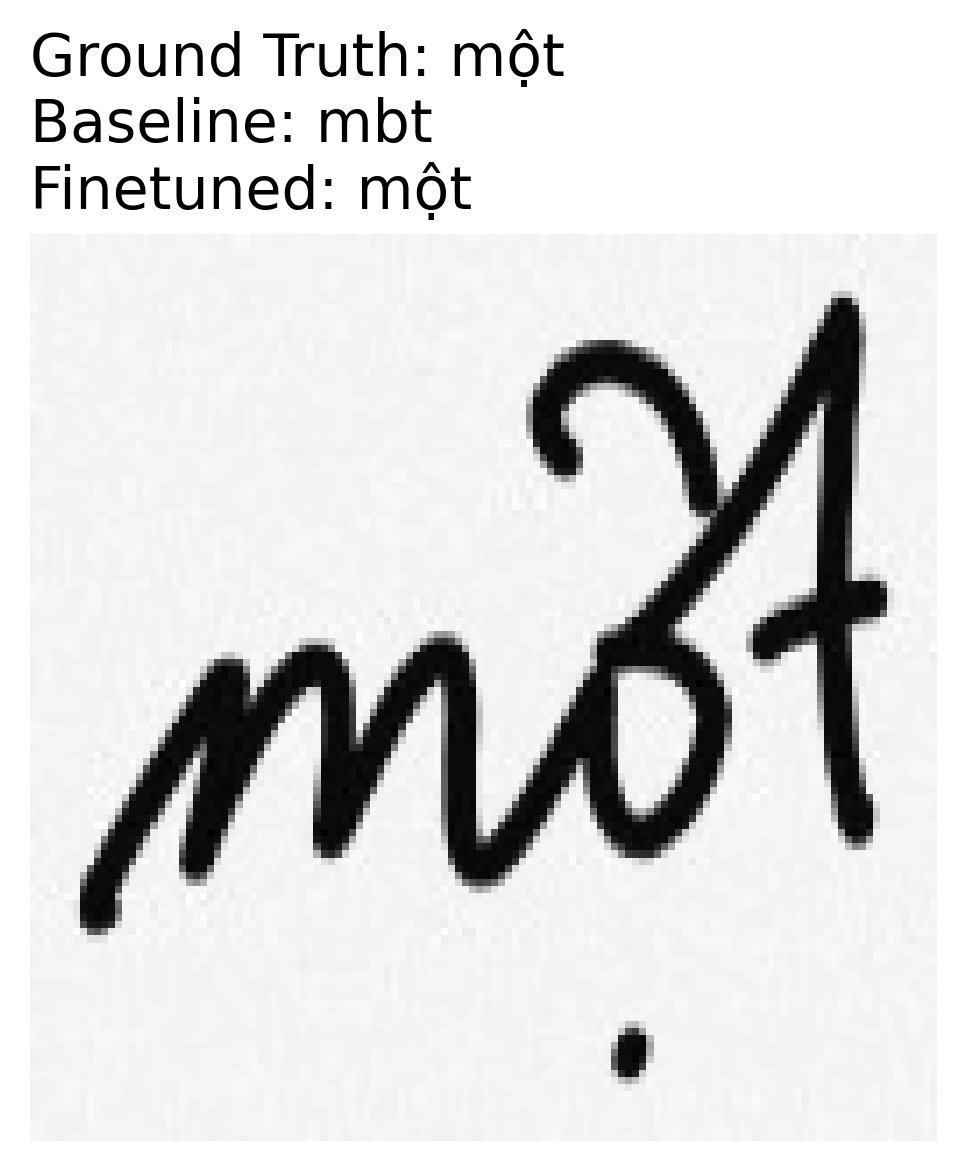
\includegraphics[width=0.6\linewidth]{img/results/improvement_example_1.png}
    \caption{Trường hợp mà mô hình Fine-tuned nhận dạng được các dấu tiếng Việt chính xác hơn so với mô hình Baseline.}
    \label{fig:improvement_1}
\end{figure}

\begin{figure}[H]
    \centering
    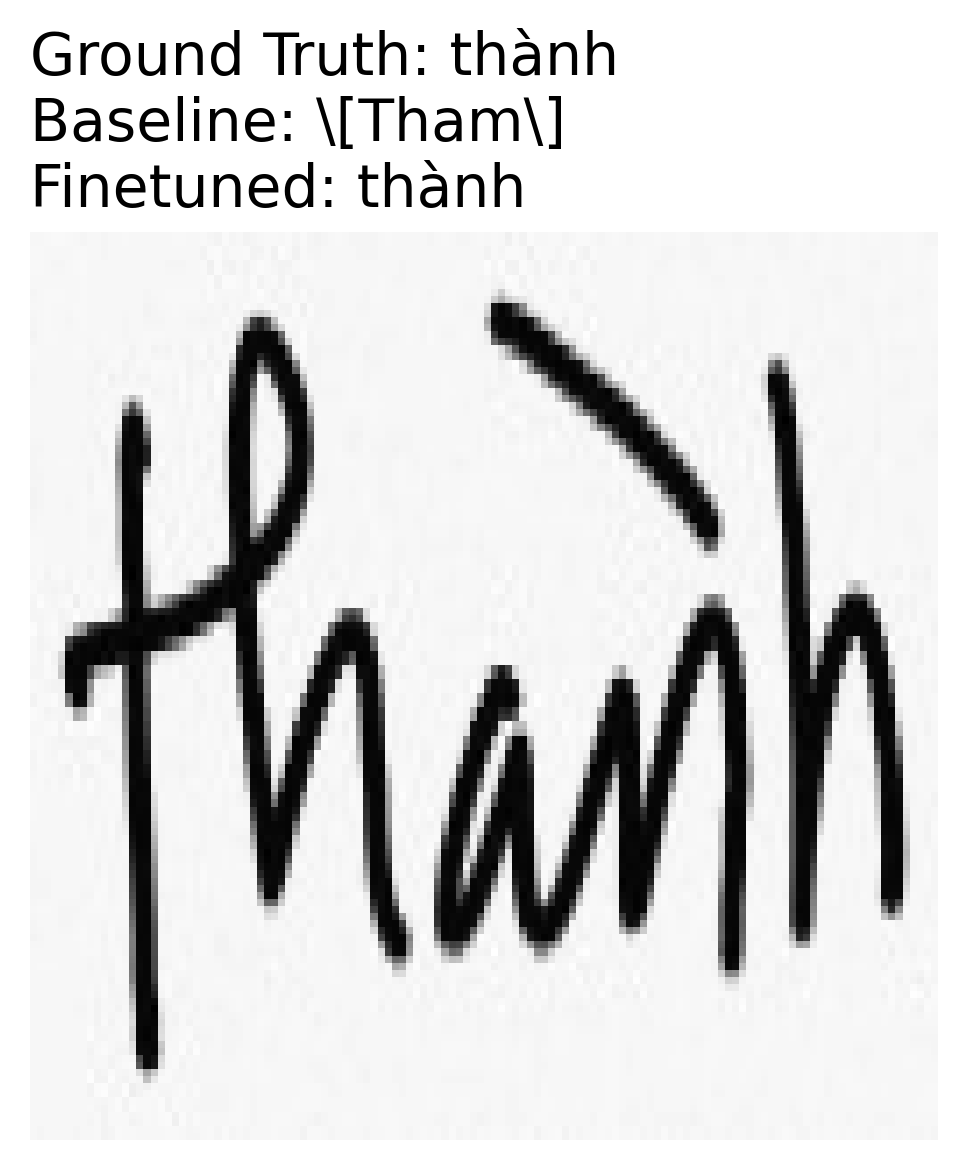
\includegraphics[width=0.6\linewidth]{img/results/improvement_example_2.png}
    \caption{Trường hợp cho thấy mô hình Fine-tuned xử lí nét viết tay phức tạp tốt hơn mô hình Baseline.}
    \label{fig:improvement_2}
\end{figure}

\begin{figure}[H]
    \centering
    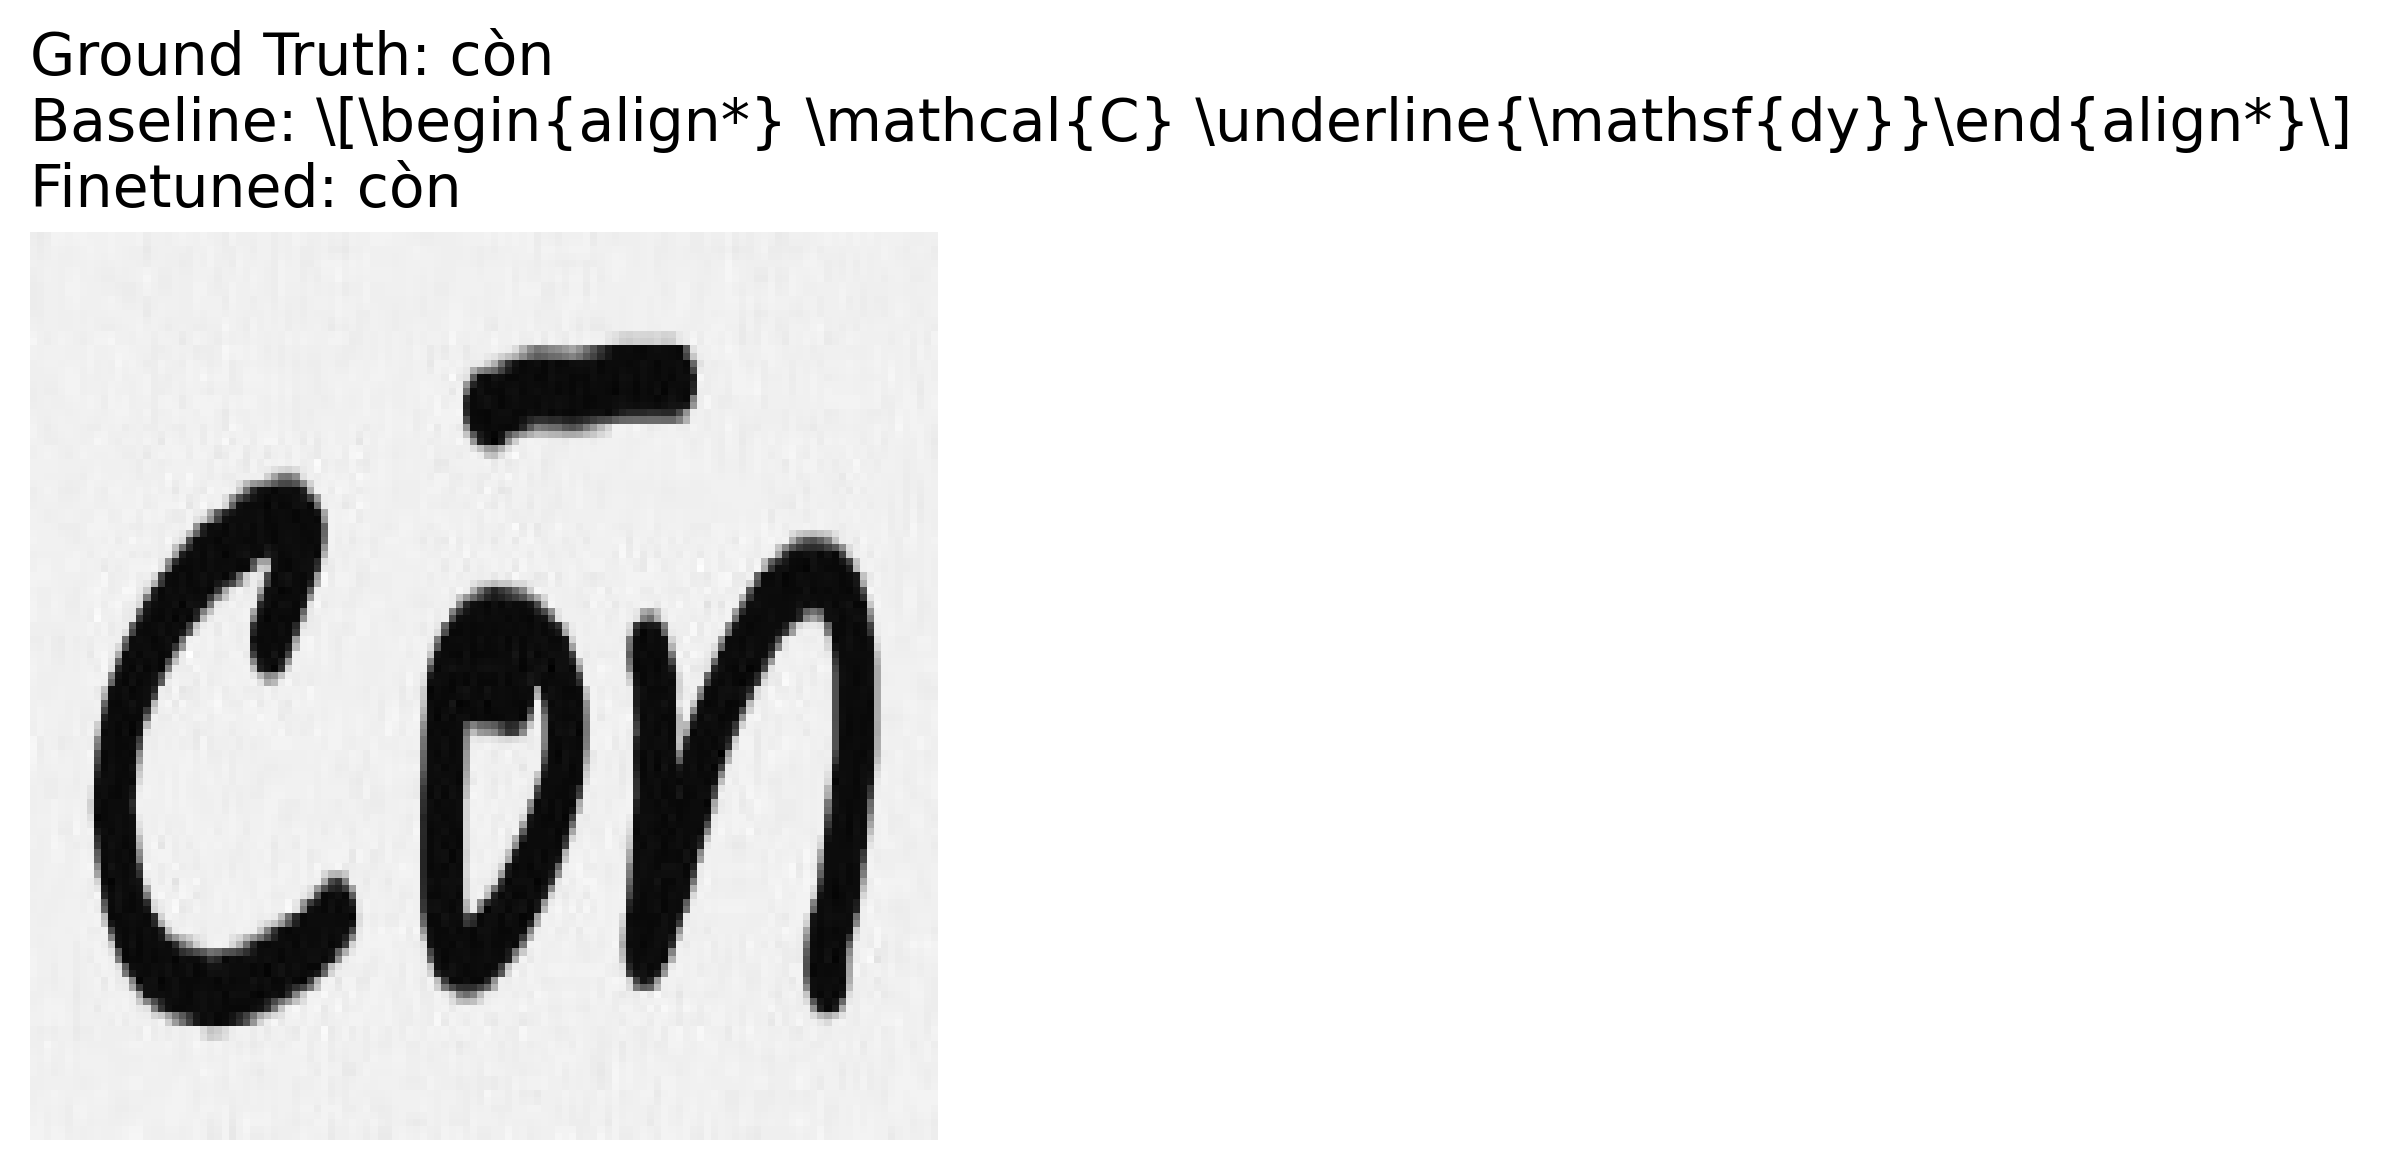
\includegraphics[width=0.8\linewidth]{img/results/improvement_example_3.png}
    \caption{Trường hợp cho thấy lỗi của mô hình Baseline được khắc phục hoàn toàn bởi mô hình Fine-tuned}
    \label{fig:improvement_3}
\end{figure}

\subsubsection{Các trường hợp lỗi còn tồn tại}
Mặc dù đạt kết quả khả quan, mô hình vẫn còn gặp một số lỗi trong các trường hợp khó:
\begin{itemize}
    \item \textbf{Nhầm lẫn các ký tự tương đồng:} Một số cặp ký tự có hình dạng viết tay rất giống nhau (như 'u' và 'n', 'h' và 'k') đôi khi vẫn bị nhận dạng sai nếu ngữ cảnh không rõ ràng.
    \item \textbf{Ảnh chất lượng thấp:} Đối với các ảnh quá mờ hoặc nhiễu nặng, mô hình có thể sinh ra các ký tự ảo (hallucination) hoặc bỏ sót ký tự.
\end{itemize}

Hình dưới đây là ví dụ điển hình về các trường hợp lỗi còn tồn tại liên quan đến nét viết tay quá tháu và nhầm lẫn ký tự:

\begin{figure}[H]
    \centering
    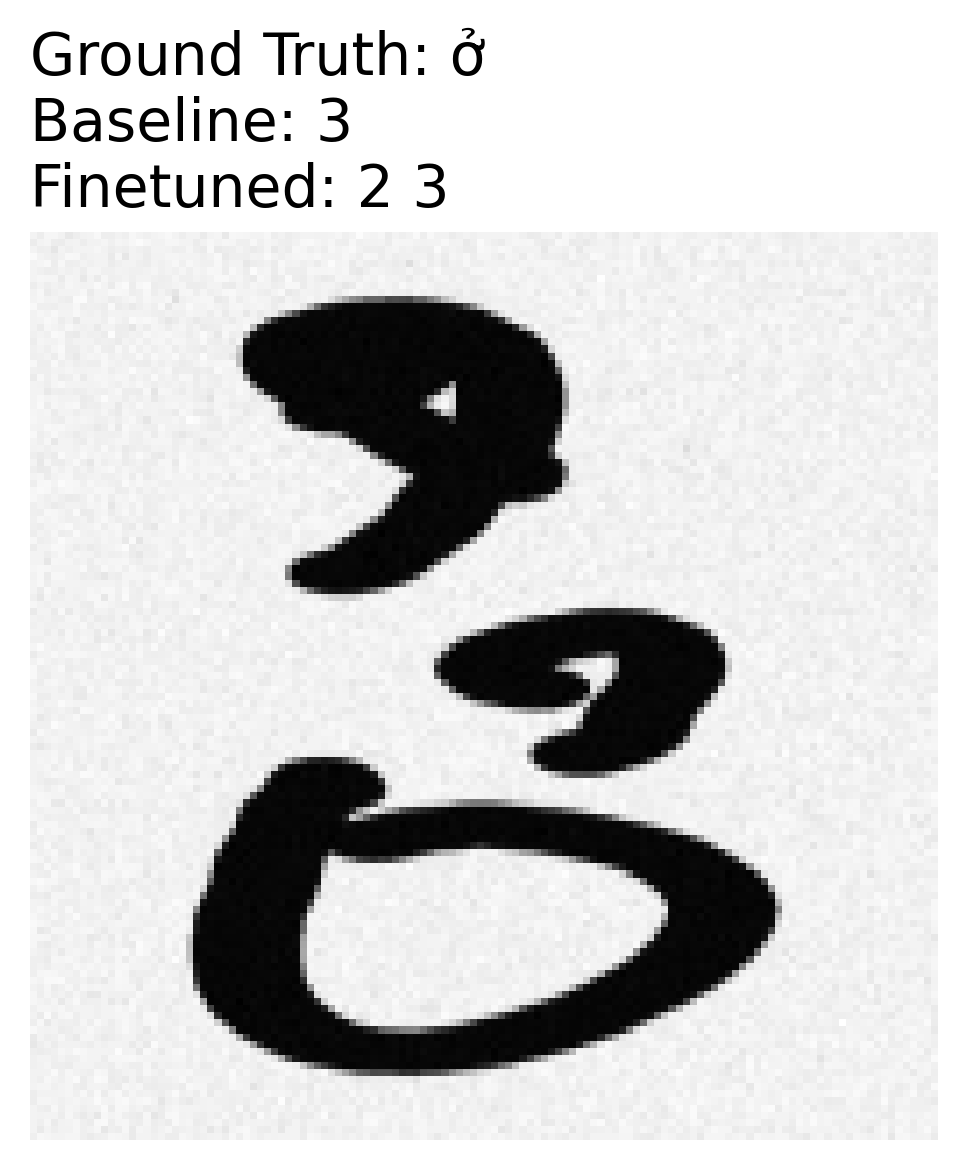
\includegraphics[width=0.4\linewidth]{img/results/worst_case_example_2.png}
    \caption{Trường hợp cho thấy mô hình fine-tuned vẫn gặp khó khăn với ảnh có chữ viết tay quá mờ và nét viết tháu. Hơn nữa, mô hình fine-tuned còn đạt được kết quả thấp hơn so với mô hình baseline trong ví dụ này.}
    \label{fig:worst_case_2}
\end{figure}